
\documentclass[12pt]{article}

\usepackage{geometry}
\geometry {
	a4paper,
	left=1cm,
	right=1cm,
	top=1cm,
	bottom=1cm
}

% Sprache, Kodierung
\usepackage[german]{babel}  % Silbentrennung ("Table of Contents" --> "Inhaltsverzeichnis")
\usepackage[utf8]{inputenc}  % Umlaute
\usepackage[T1]{fontenc}

% Farben
\usepackage{xcolor}
\usepackage[colorlinks=true, urlcolor=mailblue]{hyperref}

\definecolor{mailblue}{RGB}{6,69,173}
\definecolor{mygreen}{rgb}{0,0.6,0}
\definecolor{deepgreen}{rgb}{0,0.7,0}
\definecolor{mygray}{rgb}{0.5,0.5,0.5}
\definecolor{mymauve}{rgb}{0.58,0,0.82}
\definecolor{deepred}{rgb}{0.6,0,0}

\usepackage{array}
\usepackage{tikz}
\usetikzlibrary{positioning,automata}

% Abkürzungsverzeichnis
\usepackage{suffix}
\usepackage{xstring}
\usepackage[printonlyused, withpage]{acronym}
    
\usepackage{filecontents}
\usepackage{datatool}
\usepackage{amsmath}
\usepackage{amssymb}
\usepackage{mathabx}  % diameter (avg) symbol
\usepackage{textcomp}
\usepackage{tikz}
\usepackage{pgfgantt}
\usepackage{float}
\usepackage{calc}
\usepackage[symbol]{footmisc}
\usepackage{graphicx}

\usepackage{pgfplots}
\pgfplotsset{width=7cm, compat=1.5, table/search path={Data}}
% Preamble: \pgfplotsset{,compat=1.16}

\usepackage{caption}

% Main-Title
\newcommand\maintitle[2]{
	\begin{center}
		\textbf{{\Huge\textsc{#1}}}\\
		\vspace{-0.2cm}
		\rule{0.7\textwidth}{3pt}\\
		\vspace{0.2cm}
		{\large #2}\\
	\end{center}
}

% subsubsubsection
\newcommand
\ssss[1] {\medskip\noindent\textsc{\textbf{#1\medskip}}}

% Header
\newcommand\newtitle[1]{
	%\textrule{0.5pt}
	
	%\vspace{-0.3cm}
	{\noindent\bigskip\Large\bf\scshape #1}
	
	\vspace{-0.7cm}
	\textrule{0.5pt}
	\vspace{-0.5cm}
}

% Anführungs- und Schlusszeichen
\newcommand
\quotes[1] {\flqq #1\frqq}

% Horizontale Linie
\usepackage[normalem]{ulem}
\newcommand
\textrule[1] {
	\noindent
	\rule{\textwidth}{#1}
}

% Abbildung (Caption)
\newcommand
\abb[1] {
	\begin{quotation}
		\vspace{-0.8cm}
		\noindent\caption{#1}
	\end{quotation}
}

% Erster Buchstabe eines neuen Kapitels
\usepackage{lettrine}
\newcommand\fl[1] {
	\lettrine[lraise=0.05, nindent=0em, slope=-.5em]{#1}{}{}
}
\newcommand\fls[1] {
	\lettrine[lines=2]{#1}{}{}
}

% Listen
\renewcommand{\labelitemi}{$\blacktriangleright$}
\renewcommand{\labelitemii}{$\diamond$}
\renewcommand{\labelitemiii}{$\triangleright$}
\renewcommand{\labelitemiv}{$\ast$}
\newcommand{\litem}{\text{-}}  % Literaturverzeichnis
\usepackage{enumitem}

% TOC
\usepackage{tocloft}
\setlength\cftparskip{0pt}
\setlength\cftbeforesecskip{3pt}
\setlength\cftaftertoctitleskip{6pt}

% Head/Foot
%\usepackage{fancyhdr}
%\usepackage{extramarks}
%\pagestyle{fancy}
%\fancyhf{} % alle Kopf- und Fusszeilenfelder bereinigen
%\fancyhead[L]{\textsc{\firstleftmark}}
%\fancyhead[C]{}
%\fancyhead[R]{\slshape\rightmark}
%\renewcommand\sectionmark[1]{
%	\markboth{\thesection\ #1}{}
%}
%\fancyfoot[C]{\thepage} % Seitenzahl
%%\renewcommand{\footrulewidth}{0.4pt}
%\renewcommand\headrule{{
%	\color{black}
%	\hrule height 2pt width\headwidth
%	\vspace{1pt}
%	\hrule height 1pt width\headwidth
%	\vspace{-4pt}
%}}

\DeclareCaptionFont{CaptionFontSize}{\fontsize{10pt}{12pt}\selectfont}
\captionsetup{font=CaptionFontSize}
		

\newcommand{\code}[1]{\texttt{#1}}

% Code
\usepackage{listings}  % Darstellung von Code mit Syntaxhighlighting
\usepackage{setspace}
\usepackage{color}

\DeclareFixedFont{\ttb}{T1}{txtt}{bx}{n}{8} % for bold
\DeclareFixedFont{\ttm}{T1}{txtt}{m}{n}{8}  % for normal

\lstset{
  backgroundcolor=\color{white},   % choose the background color; you must add \usepackage{color} or \usepackage{xcolor}; should come as last argument
  basicstyle=\ttm,        % the size of the fonts that are used for the code
  breakatwhitespace=false,         % sets if automatic breaks should only happen at whitespace
  breaklines=true,                 % sets automatic line breaking
  captionpos=b,                    % sets the caption-position to bottom
  commentstyle=\color{mygreen},    % comment style
  deletekeywords={...},            % if you want to delete keywords from the given language
  escapeinside={\%*}{*)},          % if you want to add LaTeX within your code
  extendedchars=true,              % lets you use non-ASCII characters; for 8-bits encodings only, does not work with UTF-8
  firstnumber=1,                % start line enumeration with line 1000
  frame=tb,	                   % adds a frame around the code
  keepspaces=true,                 % keeps spaces in text, useful for keeping indentation of code (possibly needs columns=flexible)
  keywordstyle=\color{blue},       % keyword style
  language=Python,                 % the language of the code
  morekeywords={*,...},            % if you want to add more keywords to the set
  otherkeywords={self, None, True, False, with},  
  numbers=left,                    % where to put the line-numbers; possible values are (none, left, right)
  numbersep=5pt,                   % how far the line-numbers are from the code
  numberstyle=\tiny\color{mygray}, % the style that is used for the line-numbers
  rulecolor=\color{black},         % if not set, the frame-color may be changed on line-breaks within not-black text (e.g. comments (green here))
  showspaces=false,                % show spaces everywhere adding particular underscores; it overrides 'showstringspaces'
  showstringspaces=false,          % underline spaces within strings only
  showtabs=false,                  % show tabs within strings adding particular underscores
  stepnumber=1,                    % the step between two line-numbers. If it's 1, each line will be numbered
  stringstyle=\color{mymauve},     % string literal style
  tabsize=2,	                   % sets default tabsize to 2 spaces
  title=\lstname,                   % show the filename of files included with \lstinputlisting; also try caption instead of title
  emph={__init__, @staticmethod},          % Custom highlighting
  emphstyle=\ttb\tiny\color{deepred},    % Custom highlighting style
  stringstyle=\color{mygreen},
}


% Syntaxhighlighting for XML-code
% Source: https://tex.stackexchange.com/questions/10255/xml-syntax-highlighting
\definecolor{gray}{rgb}{0.4,0.4,0.4}
\definecolor{darkblue}{rgb}{0.0,0.0,0.6}
\definecolor{cyan}{rgb}{0.0,0.6,0.6}

\lstdefinelanguage{myXML}{
  morestring=[b]",
  morestring=[s]{>}{<},
  morecomment=[s]{<?}{?>},
  stringstyle=\color{black},
  identifierstyle=\color{darkblue},
  keywordstyle=\color{cyan},
  morekeywords={xmlns,version,type}
}

\lstset{
  literate={ö}{{\"o}}1
           {ä}{{\"a}}1
           {ü}{{\"u}}1
}

% Links
\PassOptionsToPackage{hyphens}{url}
\usepackage{hyperref}
\hypersetup{
    pdftoolbar=true,
    pdfmenubar=true,
    pdffitwindow=false,
    pdfstartview={FitH},
    pdftitle={title},
    pdfauthor={Bernard Schroffenegger},
    pdfsubject={Korpusversionen},
    pdfcreator={Bernard Schroffenegger},
    pdfproducer={Bernard Schroffenegger},
    pdfkeywords={Korpus} {Korpora} {Vergleich} {Versionen} {Werkzeug},
    pdfnewwindow=true,
    colorlinks,
    linkcolor={blue!50!black},
    citecolor={blue!50!black},
    urlcolor={blue!80!black},
	filecolor=magenta
}


% \usepackage{breakurl}

% Fussnoten
\renewcommand{\thefootnote}{\arabic{footnote}}

% Symbol über und unter "=":
% https://tex.stackexchange.com/questions/123219/writing-above-and-below-a-symbol-simultaneously, 6.5.2019
\usepackage{stackengine}
\newcommand\stackequal[2]{%
  \mathrel{\stackunder[2pt]{\stackon[4pt]{$\Rightarrow$}{$\scriptscriptstyle#1$}}{%
  $\scriptscriptstyle#2$}}}

% Tabellen
\usepackage{multirow}

\tikzstyle{bag} = [align=center]

% Bilder
\usepackage{caption}
\usepackage{subcaption}

% Tabellen
\usepackage{booktabs}  % toprule, midrule, bottomrule, \cmidrule{...}, ...
\usepackage{wasysym}
\newenvironment{rcases}
  {\left.\begin{aligned}}
  {\end{aligned}\right\rbrace}
\usepackage{nicefrac}
\usepackage{pifont}% http://ctan.org/pkg/pifont
\newcommand{\cmark}{\ding{51}}%
\newcommand{\xmark}{\ding{55}}%

\begin{document}

\begin{center}
\noindent
{\LARGE \textsc{\textbf{Optical Character Recognition (OCR)}}}\\
\vspace*{-0.cm}
%\rule{0.9\textwidth}{1pt}\\
\vspace*{0.1cm}
{\LARGE \textsc{\textbf{with ABBYY FineReader \& Kraken}}}\\

\vspace*{-0.2cm}
\rule{0.75\textwidth}{2pt}\\
\vspace*{-0.0cm}
{
	\textbf{Institute for Computational Linguistics, 2020}\\
}

\begin{quote}
\textbf{Abstract:} This paper briefly summarizes the applied OCR methods as well as the (optional) file splitting in the digitalization process of 10'012 file cards, given as pages in one large pdf file (778.8 MB).
\end{quote}

\end{center}



\noindent
\section{Preprocessing}

\noindent
Breaking the input into multiple pieces is not necessarily needed, however, \quotes{divide et impera} appears to be a recommendable strategy: A preceding splitting bewares from reprocessing everything in case of an error, and might, facilitating parallelization, speed up the process significantly.

\medskip

\vspace*{-0.1cm}
\begin{quote}
\begin{lstlisting}
from PyPDF2 import PdfFileWriter, PdfFileReader
input_pdf = PdfFileReader(open("/path/to/input/file.pdf", "rb"))
for i in range(input_pdf.numPages):
    with open("file_"+(5-len(str(i+1)))*'0'+str(i+1)+".pdf", "wb") as output:
        PdfFileWriter().addPage(input_pdf.getPage(i)).write(output)
\end{lstlisting}
\begin{center}
\vspace*{-1.4cm}
Code Snipped: A Python-script to save each page of a pdf file as a new pdf file.
\end{center}
\end{quote}

The names of the output files should be of uniform length (depending on the particular naming system). Otherwise, $abc$-sort of certain file explorers might destroy the order, which eventually has disadvantageous effects on further processing steps (e.g. required id-extraction from file names).

\section{ABBYY FineReader}

This section documents the process of applying OCR on multiple files by the commercially proprietary software \quotes{FineReader} by ABBYY, which involves the creation of different directories as well as some configuration steps.

\subsection{Directories (Input/Output)}

FineReader requires up to 5 directories (R/W rights required):

\vspace*{-0.1cm}
\begin{itemize}
\setlength\itemsep{0em}
\item Input (\quotes{Hot Folder})
\item Output (the OCR output in its desired format)
\item Errors (corrupt input files and corresponding log files)
\item Log files (optional)
\item Images (optional; the input after passing the \quotes{Hot Folder})
\end{itemize}


\subsection{Configuration}

The entire process can be defined in a single \quotes{Workflow}:

\vspace*{0.3cm}
\begin{minipage}{0.4\textwidth} 
\begin{center}
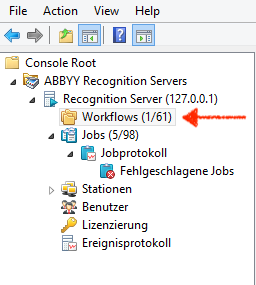
\includegraphics[scale=0.7]{main.png}
\end{center}
\end{minipage}
\begin{minipage}{0.4\textwidth}
\begin{center}
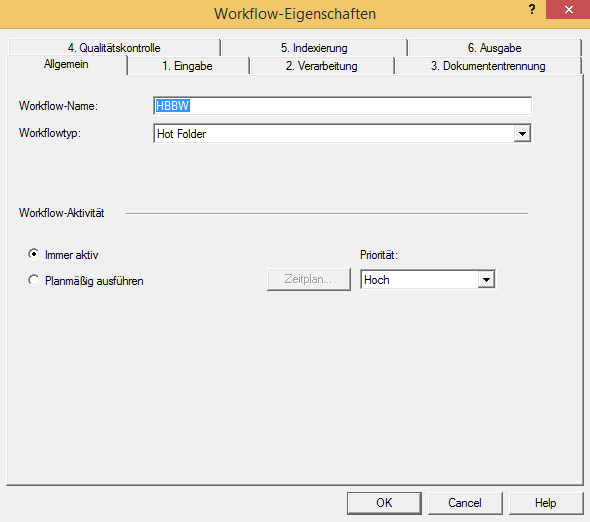
\includegraphics[scale=0.42]{0_allgemein.png}
\end{center}
\end{minipage}


\begin{minipage}{0.4\textwidth} 
\begin{center}
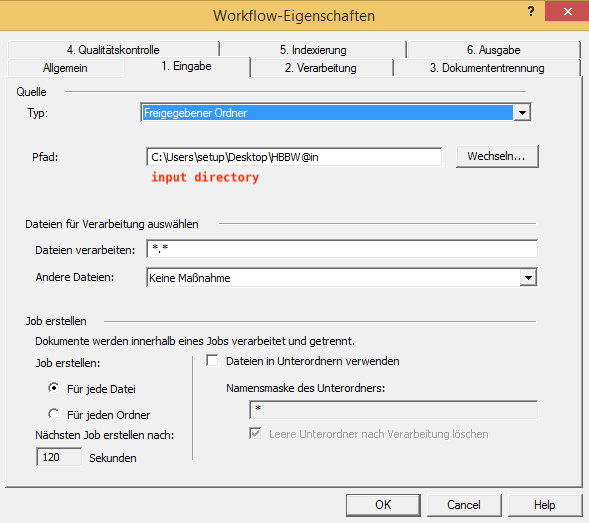
\includegraphics[scale=0.42]{1_eingabe.png}
\end{center}
\end{minipage}
\begin{minipage}{0.4\textwidth}
\begin{center}
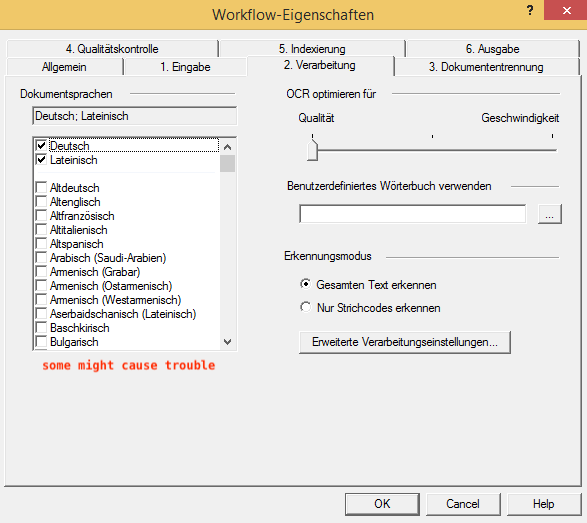
\includegraphics[scale=0.42]{2_verarbeitung.png}
\end{center}
\end{minipage}


\begin{minipage}{0.4\textwidth}
\begin{center}
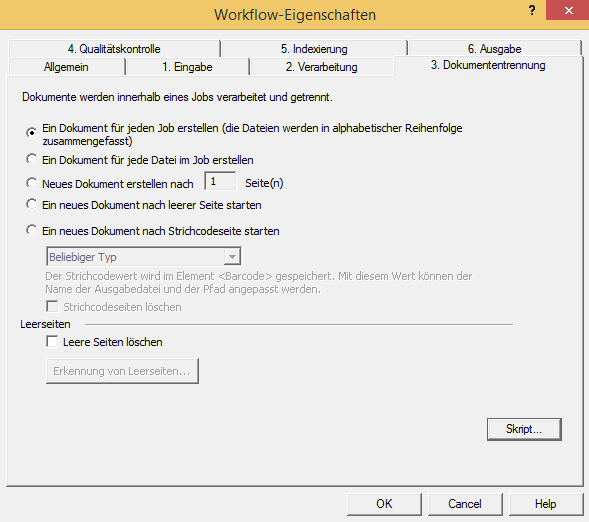
\includegraphics[scale=0.42]{3_dokumententrennung.png}
\end{center}
\end{minipage}
\begin{minipage}{0.4\textwidth}
\begin{center}
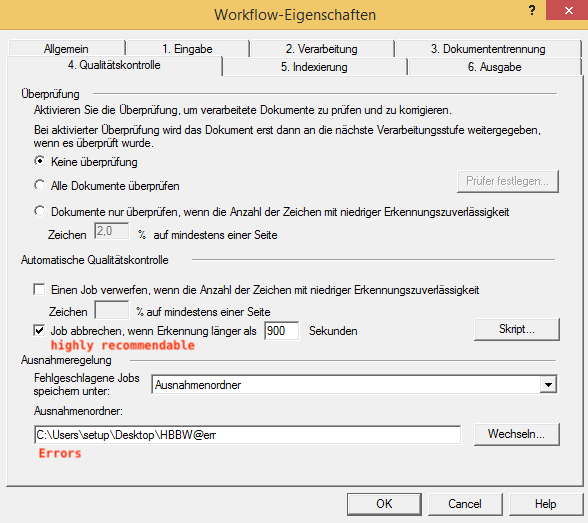
\includegraphics[scale=0.42]{4_qualitaetskontrolle.png}
\end{center}
\end{minipage}


\begin{minipage}{0.4\textwidth}
\begin{center}
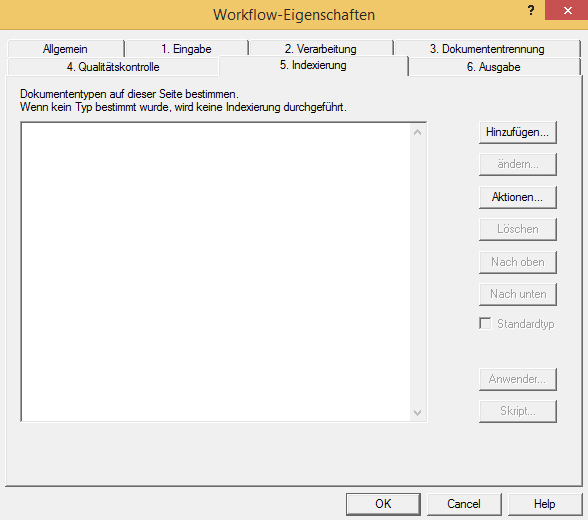
\includegraphics[scale=0.42]{5_indexierung.png}
\end{center}
\end{minipage}
\begin{minipage}{0.4\textwidth}
\begin{center}
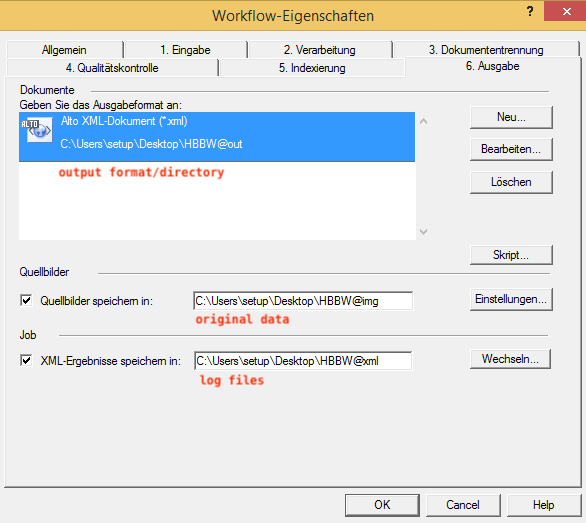
\includegraphics[scale=0.42]{6_ausgabe.png}
\end{center}
\end{minipage}


\subsection{Execution}

After completing the configuration above (by clicking on \quotes{ok}), the input directory becomes active. Every file in this directory appears to magically disappear, and (eventually) reappear again in the image directory - together with data in the other directories, as indicated by their names.
If there are no configuration problems, the output follows immediately.
Otherwise, the overviews \quotes{Jobs}, \quotes{Job Protokoll} and \quotes{Fehlgeschlagene Jobs} (see Workflow) might reveal some information about the problem.

\medskip

With the settings described, FineReader needed 3h and 49m to process our 10'012 files, thats is, 1.37s per file (80 KB) on average.

\section{Kraken}

The OCR-Tool \quotes{Kraken} needs to be downloaded and installed as described on the \href{http://kraken.re/}{official website} or on \href{https://github.com/mittagessen/kraken}{GitHub}. Since Kraken runs on images, our pdf files had to be transformed first:

\begin{quote}
\begin{lstlisting}
from pdf2image import convert_from_path
for page in convert_from_path("path/to/input_file.pdf", 300):  # dpi
	  page.save("path/to/output_file.png", 'PNG')
\end{lstlisting}
\vspace{-1.cm}
\begin{center}
Code Snipped (Python): pdf $\rightarrow$ png
\end{center}
\end{quote}

\begin{quote}
\begin{lstlisting}
import subprocess, psutil
def run_kraken(input_path_png, output_path):
	  cmd, url_model = "binarize segment ocr -a -m", "path/to/language_best.mlmodel"
	  cmd = ' '.join(["kraken -i", input_path_png, output_path, cmd, url_model])
	  sub_process = subprocess.Popen([cmd], shell=True)
	  p = psutil.Process(sub_process.pid)
	  try: p.wait(timeout=100)
	  except psutil.TimeoutExpired: p.kill()
\end{lstlisting}
\vspace{-1.cm}
\begin{center}
Code Snipped (Python): png $\rightarrow$ xml (alto)
\end{center}
\end{quote}


%\section{Postprocessing}
%
%\subsection{Scaling}
%
%The size of a page (length times width [px]) differs from file to file. Consequently, a reliable detection of contents based on absolute positions requires to normalize all coordinates.
%
%
%\begin{itemize}
%\item width $B_i$ $\propto$ $S_{i\alpha x}$(WIDTH$_{i\alpha x}$, HPOS$_{i\alpha x})$
%\item height $H_i$ $\propto$ $S_{i\alpha y}$(HEIGHT$_{i\alpha y}$, VPOS$_{i\alpha y}$)
%\end{itemize}
%
%\vspace*{-0.5cm}
%\begin{center}
%\begin{tikzpicture}[fill=blue!20, scale=0.8]
%% Koordinaten/Beschriftungen
%\draw[line width=2pt] (0,-5) -- (0,0) -- (10,0);
%% \draw (-2,0) node[anchor=south]{\scriptsize \code{page}};
%
%% Element
%\fill (2,-2) -- (6,-2) -- (6,-3) -- (2,-3) -- (2,-2);
%
%\draw[>=latex,<->] (2,0) -- (2,-2);
%\draw (2,-1) node[anchor=west]{{\tiny $VPOS_\alpha$}};
%\draw[>=latex,<->] (0,-2) -- (2,-2);
%\draw (1,-2) node[anchor=south]{{\tiny $HPOS_\alpha$}};
%\draw[>=latex,<->] (2,-3.3) -- (6,-3.3);
%\draw (4,-3.3) node[anchor=north]{{\tiny $WIDTH_\alpha$}};
%\draw[>=latex,<->] (6.3,-2) -- (6.3,-3);
%\draw (6.3,-2.5) node[anchor=west]{{\tiny $HEIGH_\alpha$}};
%
%\draw[red, densely dotted] (2,-3)--(2,-3.5);
%\draw[red, densely dotted] (6,-3)--(6,-3.5);
%\draw[red, densely dotted] (6,-3)--(6.5,-3);
%\draw[red, densely dotted] (6,-2)--(6.5,-2);
%
%\draw[dashed] (4,0)--(4,-2.5);
%\draw[dashed] (0,-2.5)--(4,-2.5);
%
%\draw (4,0) circle (2pt);
%\draw (4,-2.5) circle (2pt);
%\draw (0,-2.5) circle (2pt);
%
%\draw (4,0) node[anchor=south]{$S_{\alpha x}$};
%\draw (4,-2.5) node[anchor=west]{$S_\alpha $};
%\draw (0,-2.5) node[anchor=east]{$S_{\alpha y}$};
%
%\end{tikzpicture}
%\end{center}
%
%\vspace*{-0.9cm}
%\begin{footnotesize}
%\begin{equation*}
%\text{Scaling factors:}\quad
%x_s (B_i) = \frac{\hat{B}}{B_i},\quad
%y_s (H_i) = \frac{\hat{H}}{H_i}\quad
%(\hat{B}:=\text{norm width},\,
%\hat{H}:=\text{norm height}).
%\end{equation*}
%\end{footnotesize}
%
%
%\subsection{Parsing}
%
%\begin{lstlisting}
%import xml.sax
%import pandas as pd
%from xml.sax.handler import ContentHandler
%
%class AltoParser(ContentHandler):
%
%    """ [String, HPOS, VPOS, HEIGHT, WIDTH] --> [str, x, y, baseline] """
%
%    # filter
%    NAMES = ["Datum", "Absender", "Empfaenger", "Autograph", "Kopie", "Photokopie",
%             "Standort", "Bull.", "Corr.", "Sign.", "Abschrift", "Umfang", "Sprache",
%             "Literatur", "Gedruckt", "Bemerkungen"]s
%
%    def __init__(self, scaling, inverse=False):
%        super(AltoParser, self).__init__()
%        self.data = pd.DataFrame({'Value': [], 'x': [], 'y': [], "Baseline": []})
%        self.current_baseline = 0
%        self.scaling = scaling
%        self.inverse = inverse
%
%    def startElement(self, name, attributes):
%        if name == "TextLine":
%            for a in attributes.getNames():
%                if a == "BASELINE":
%                    self.current_baseline = attributes.getValue(a)
%
%        if name == "String" and "STYLE" not in attributes.getNames():
%            d = dict()
%            d["BASELINE"] = self.current_baseline
%            for a in attributes.getNames():
%                d[a] = attributes.getValue(a)
%            if self.inverse:
%                if d["CONTENT"] not in AltoParser.NAMES:
%                    self.append(d)
%            else:
%                if d["CONTENT"] in AltoParser.NAMES:
%                    self.append(d)
%
%    def append(self, d):
%        hpos, vpos = int(d["HPOS"]), int(d["VPOS"])
%        width, height = int(d["WIDTH"]), int(d["HEIGHT"])
%        x, y = AltoParser.get_mass_point(hpos, vpos, width, height, self.scaling)
%        value = ''
%        if ("SUBS_TYPE" in d) and ("SUBS_CONTENT" in d):
%            if d["SUBS_TYPE"] == "HypPart1":
%                value = d["SUBS_CONTENT"]
%        else: value = d["CONTENT"]
%        df = pd.DataFrame({
%            'Value': [value],
%            'x': [x], 'y': [y],
%            'Baseline': [self.current_baseline]
%        })
%        self.data = pd.concat([self.data, df])
%
%    @staticmethod
%    def get_mass_point(hpos, vpos, width, height, scaling):
%        """ text center coordinates """
%        x, y = hpos + 0.5 * width, vpos + 0.5 * height
%        return int(scaling[0]*x), int(scaling[1]*y)
%
%    @staticmethod
%    def extract_data(path, scaling, inverse=False):
%        try:
%            parser = xml.sax.make_parser()
%            counter = AltoParser(scaling, inverse=inverse)
%            parser.setContentHandler(counter)
%            parser.parse(path)
%            return counter.data
%        except:
%            print("*** Warning: alto-parser failed on", path)
%            return pd.DataFrame({'Value': [], 'x': [], 'y': [], "Baseline": []})
%\end{lstlisting}

\end{document}
